\section{AC/DC Power Circuit Application}
Trong bài tập này, chúng ta đang xây dựng từng bước chuyển đổi nguồn điện áp AC sang DC
mạch. Học sinh thực hiện mô phỏng miền thời gian và viết ra các nhận xét cũng như giải thích cho từng bước.

\textbf{Tip:} Để đặt một tụ điện, hãy đi tới  \textbf{Place > PSpice Component > Capacitor}
\begin{itemize}
    \item \textbf{Step 1:} Điện áp được chỉnh lưu mà không cần lọc hoặc điều chỉnh.
    \begin{figure}[ht]
        \centering
        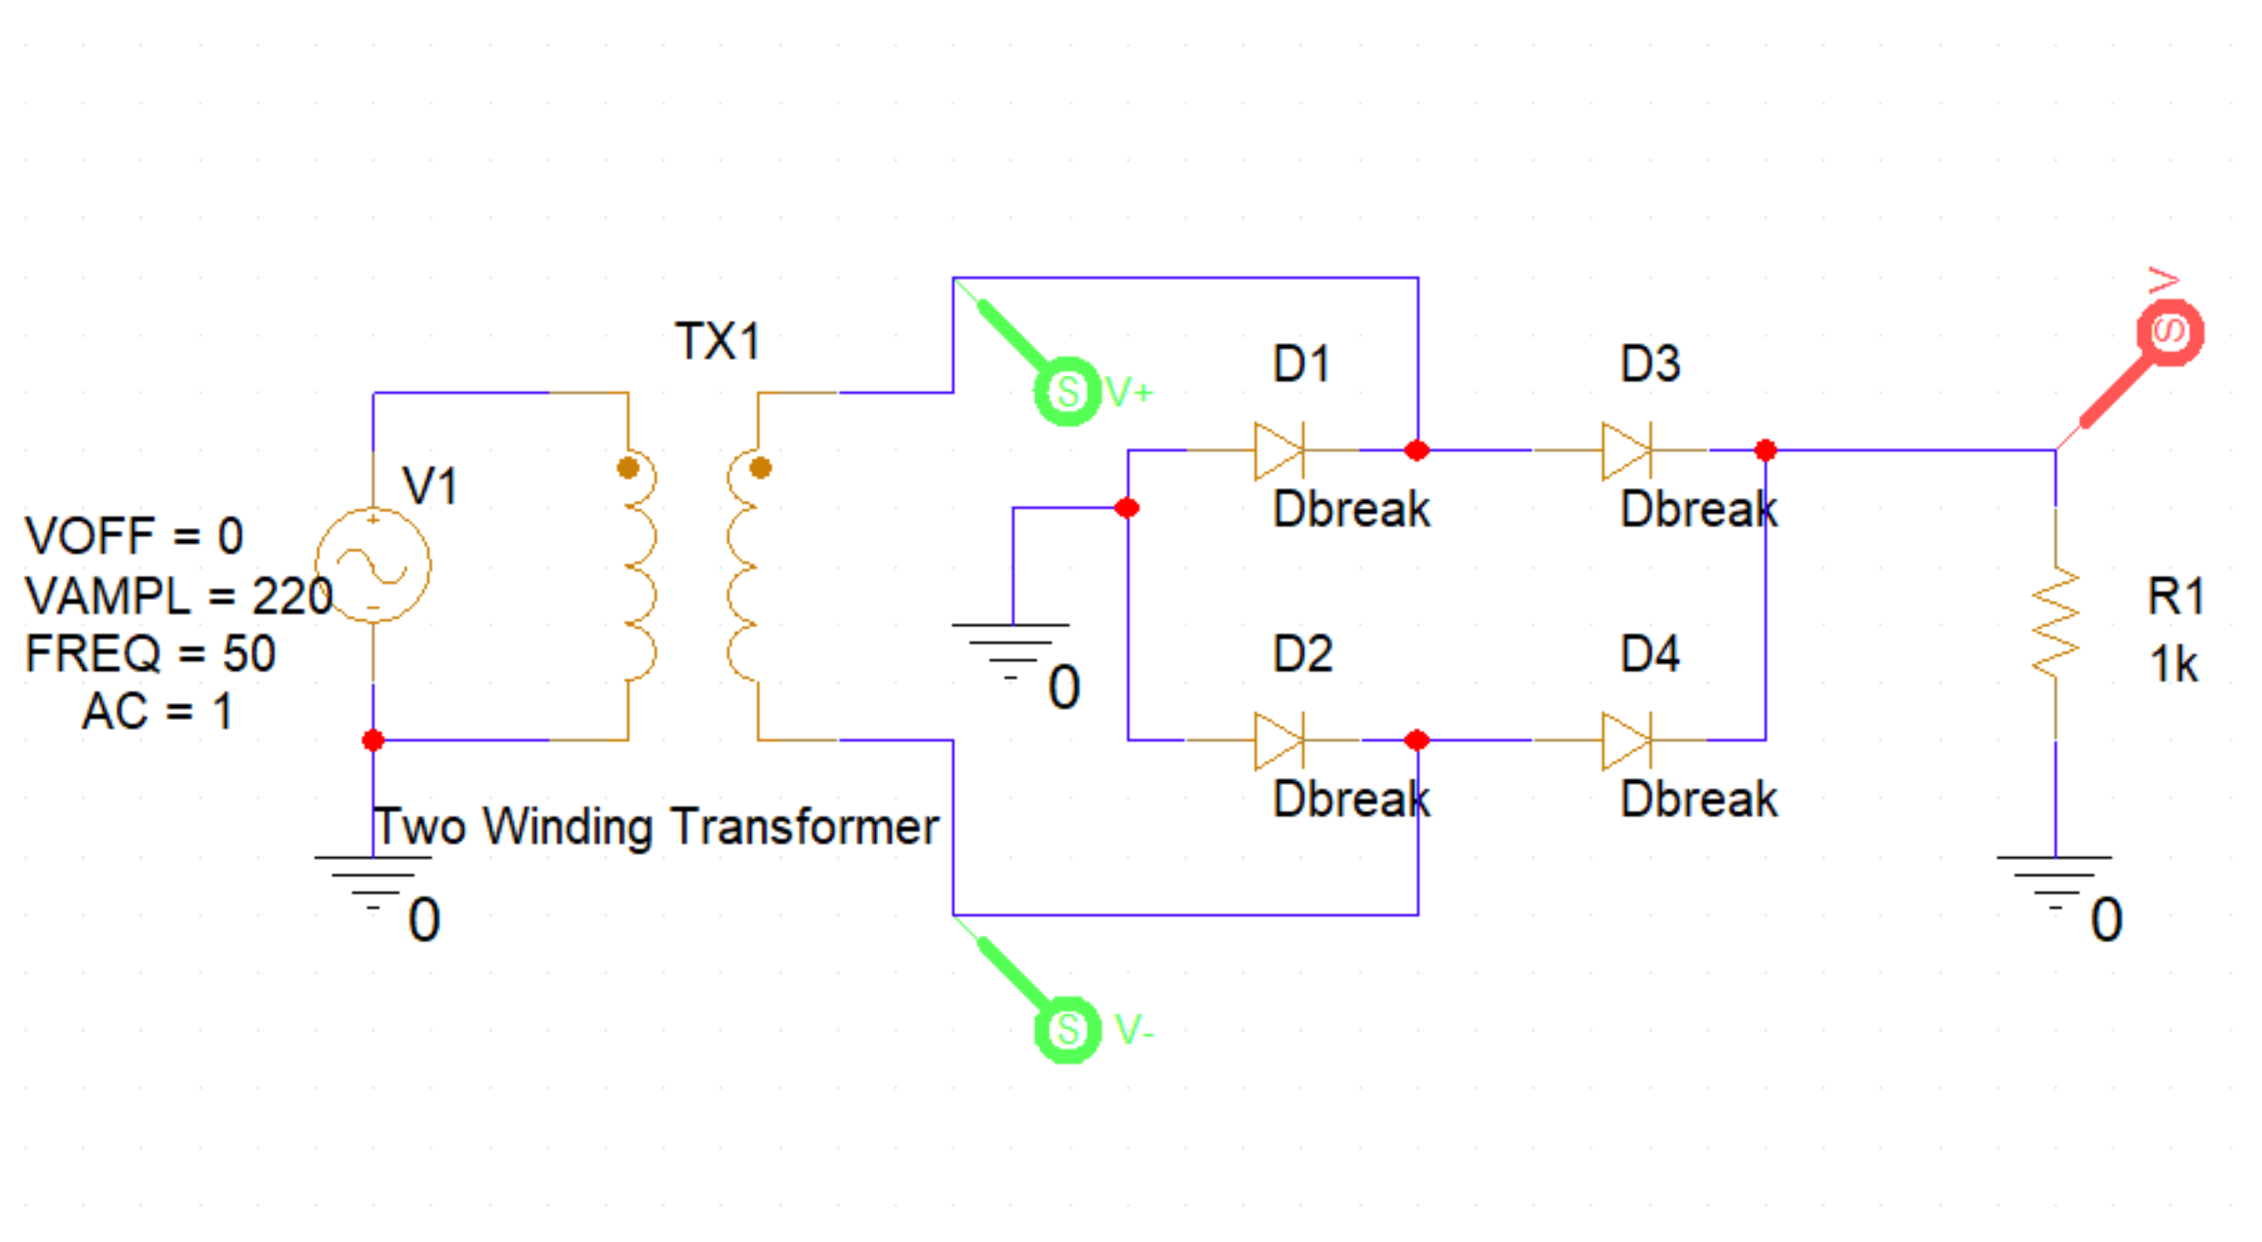
\includegraphics[scale= 0.26]{graphics/ex9/f1.png}
        \caption{Điện áp được chỉnh lưu mà không cần lọc hoặc điều chỉnh}
    \end{figure}
\pagebreak
    \textbf{Kết quả mô phỏng: }

    \begin{figure}[ht]
        \centering
        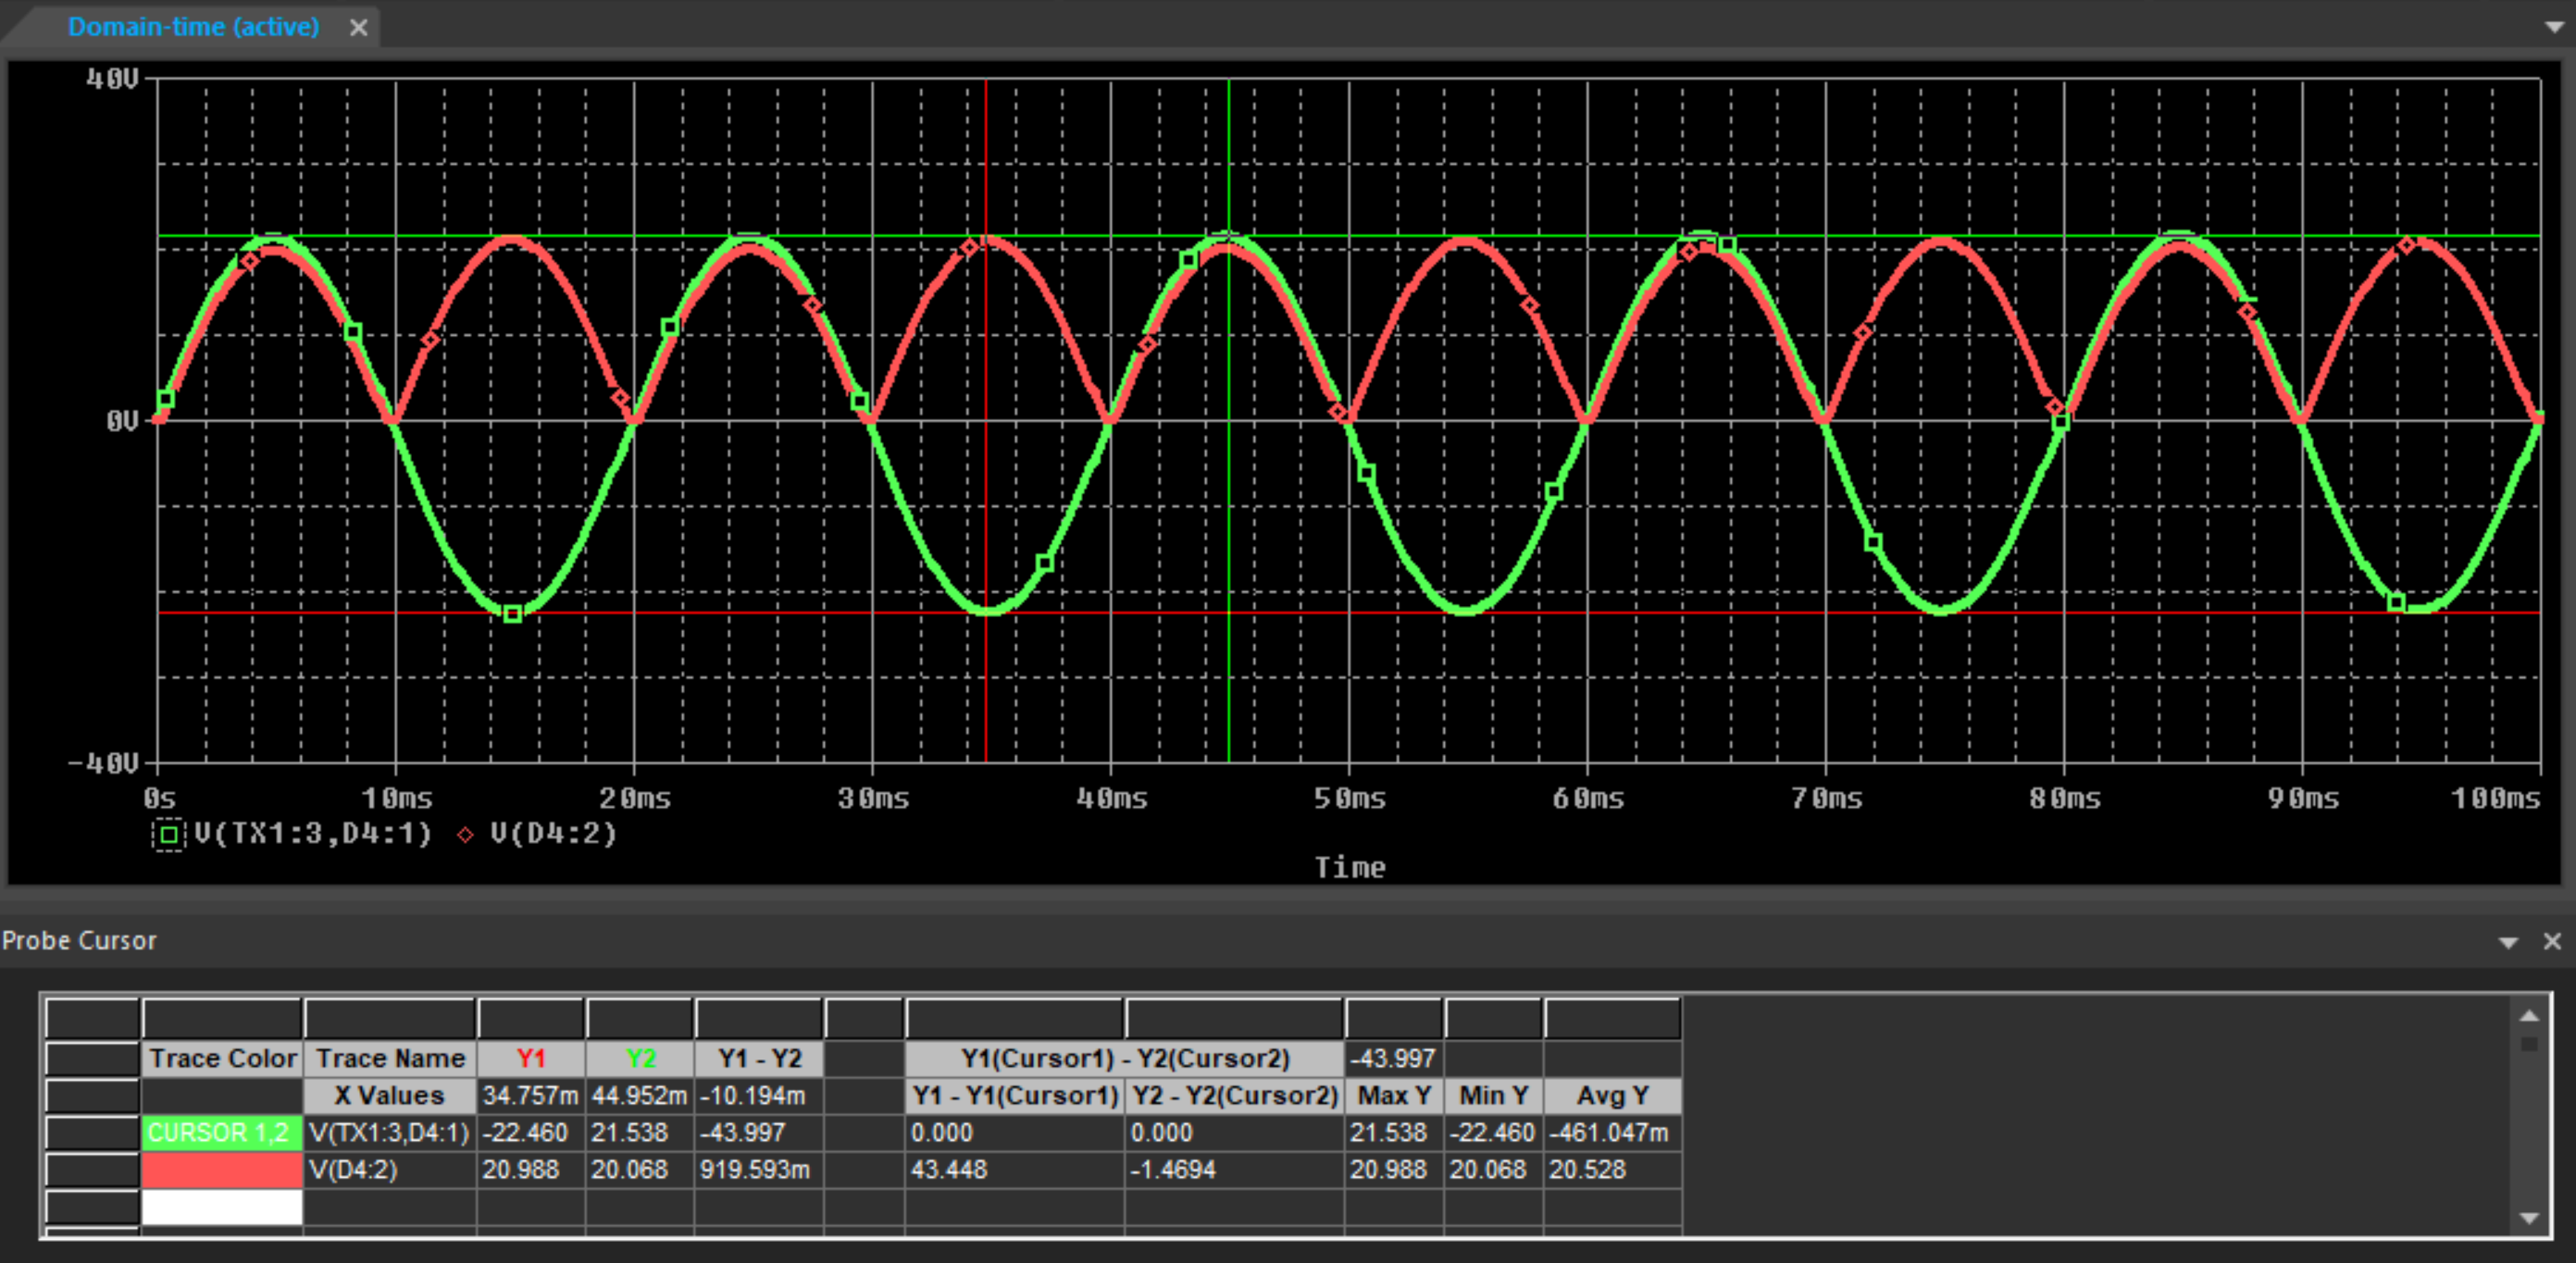
\includegraphics[scale= 0.2]{graphics/ex9/f2.png}
        \caption{Kết quả mô phỏng của mạch trong hình 9.1}
    \end{figure}

    \textbf{Ý kiến hoặc giải thích:} Đồ thị của \(V_{DC}\) qua điện trở (màu đỏ) chưa ổn định do sự chuyển pha theo chu kỳ (đồ thị hình sin trong hình)
    
    \item \textbf{Step 2:} Điện áp chỉnh lưu được điều chỉnh bằng tụ điện 10µF.
    
    \begin{figure}[ht]
        \centering
        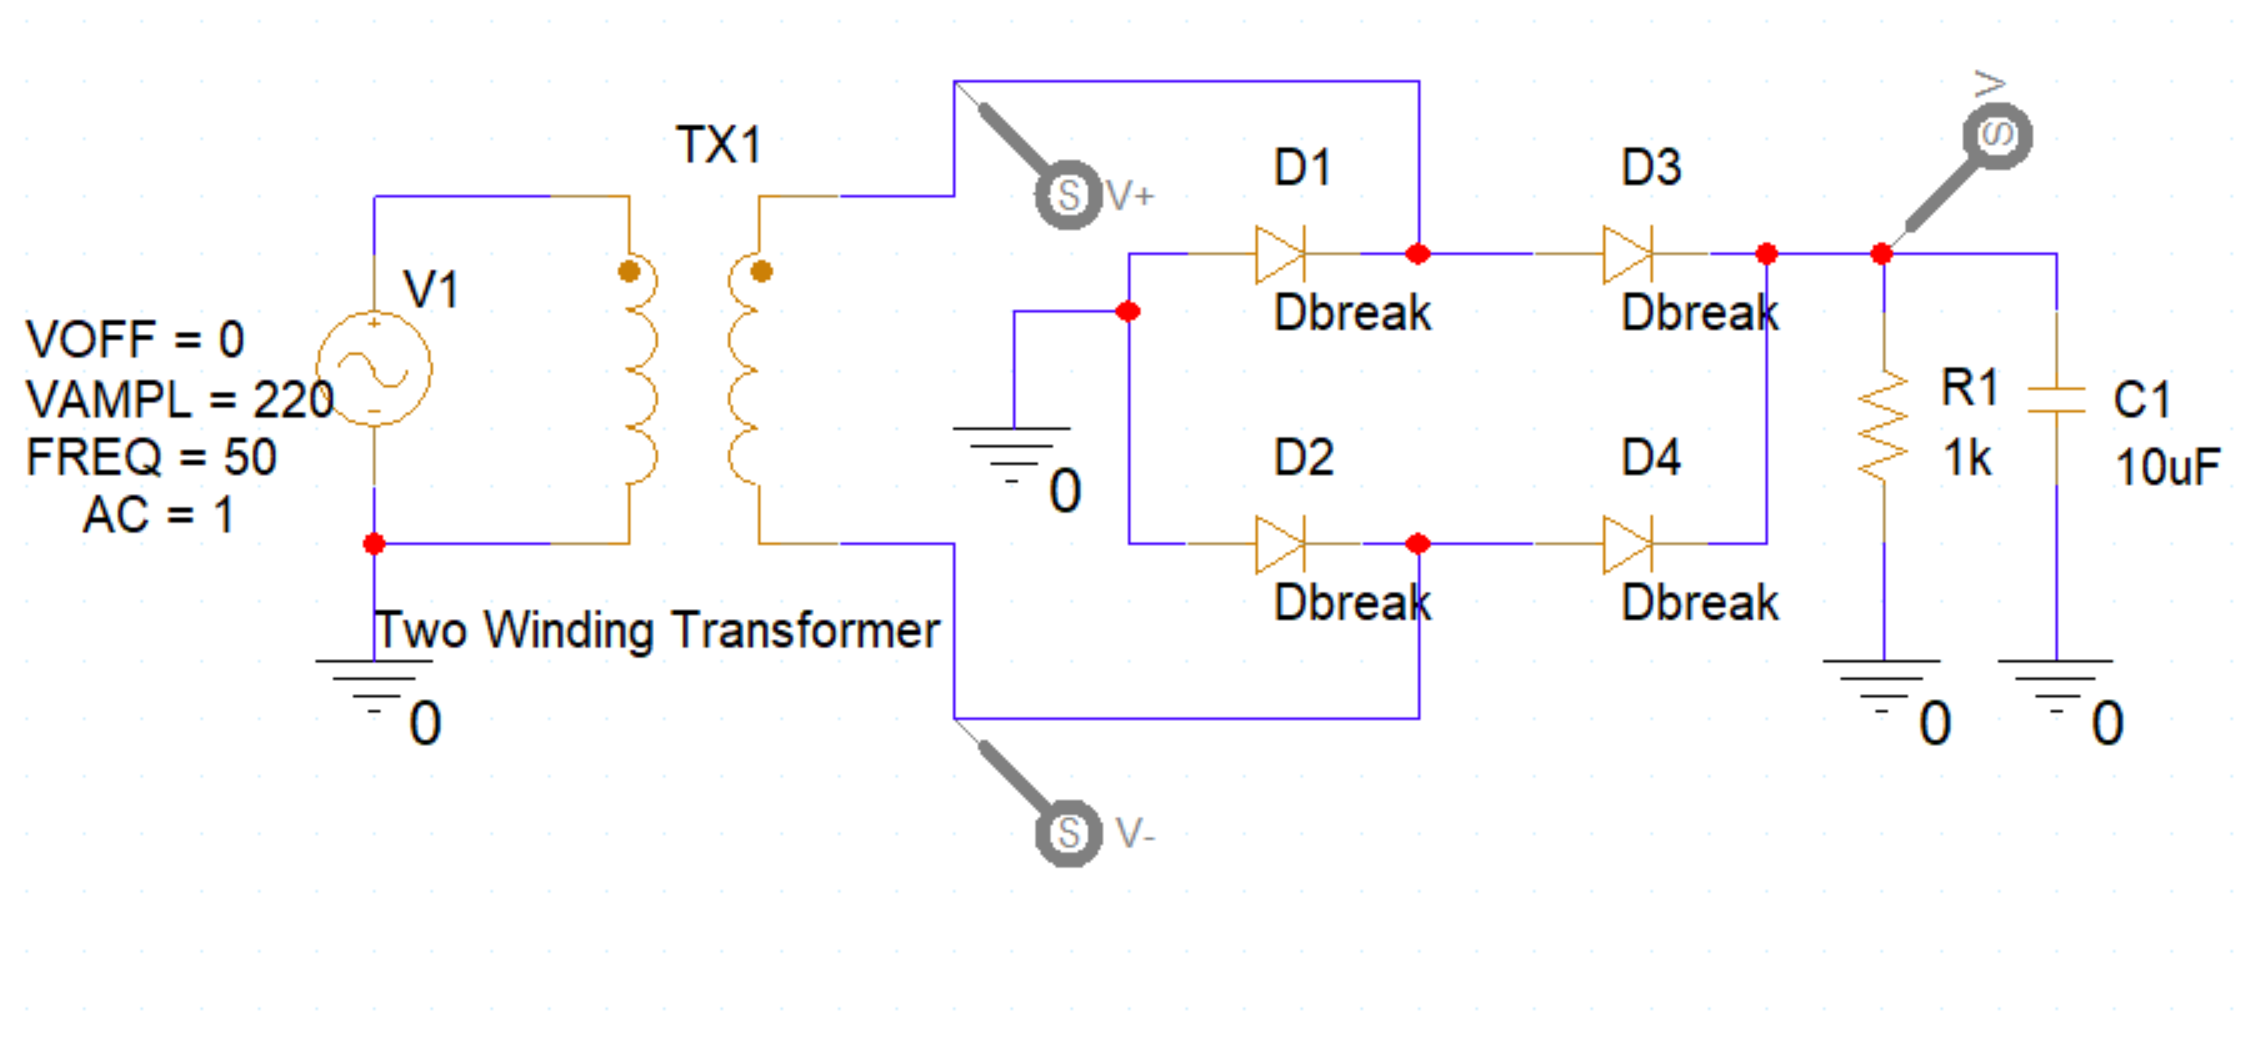
\includegraphics[scale= 0.26]{graphics/ex9/f3.png}
        \caption{Chỉnh lưu điện áp được điều chỉnh bằng tụ điện}
    \end{figure}
\pagebreak
    \textbf{Kết quả mô phỏng: }

    \begin{figure}[ht]
        \centering
        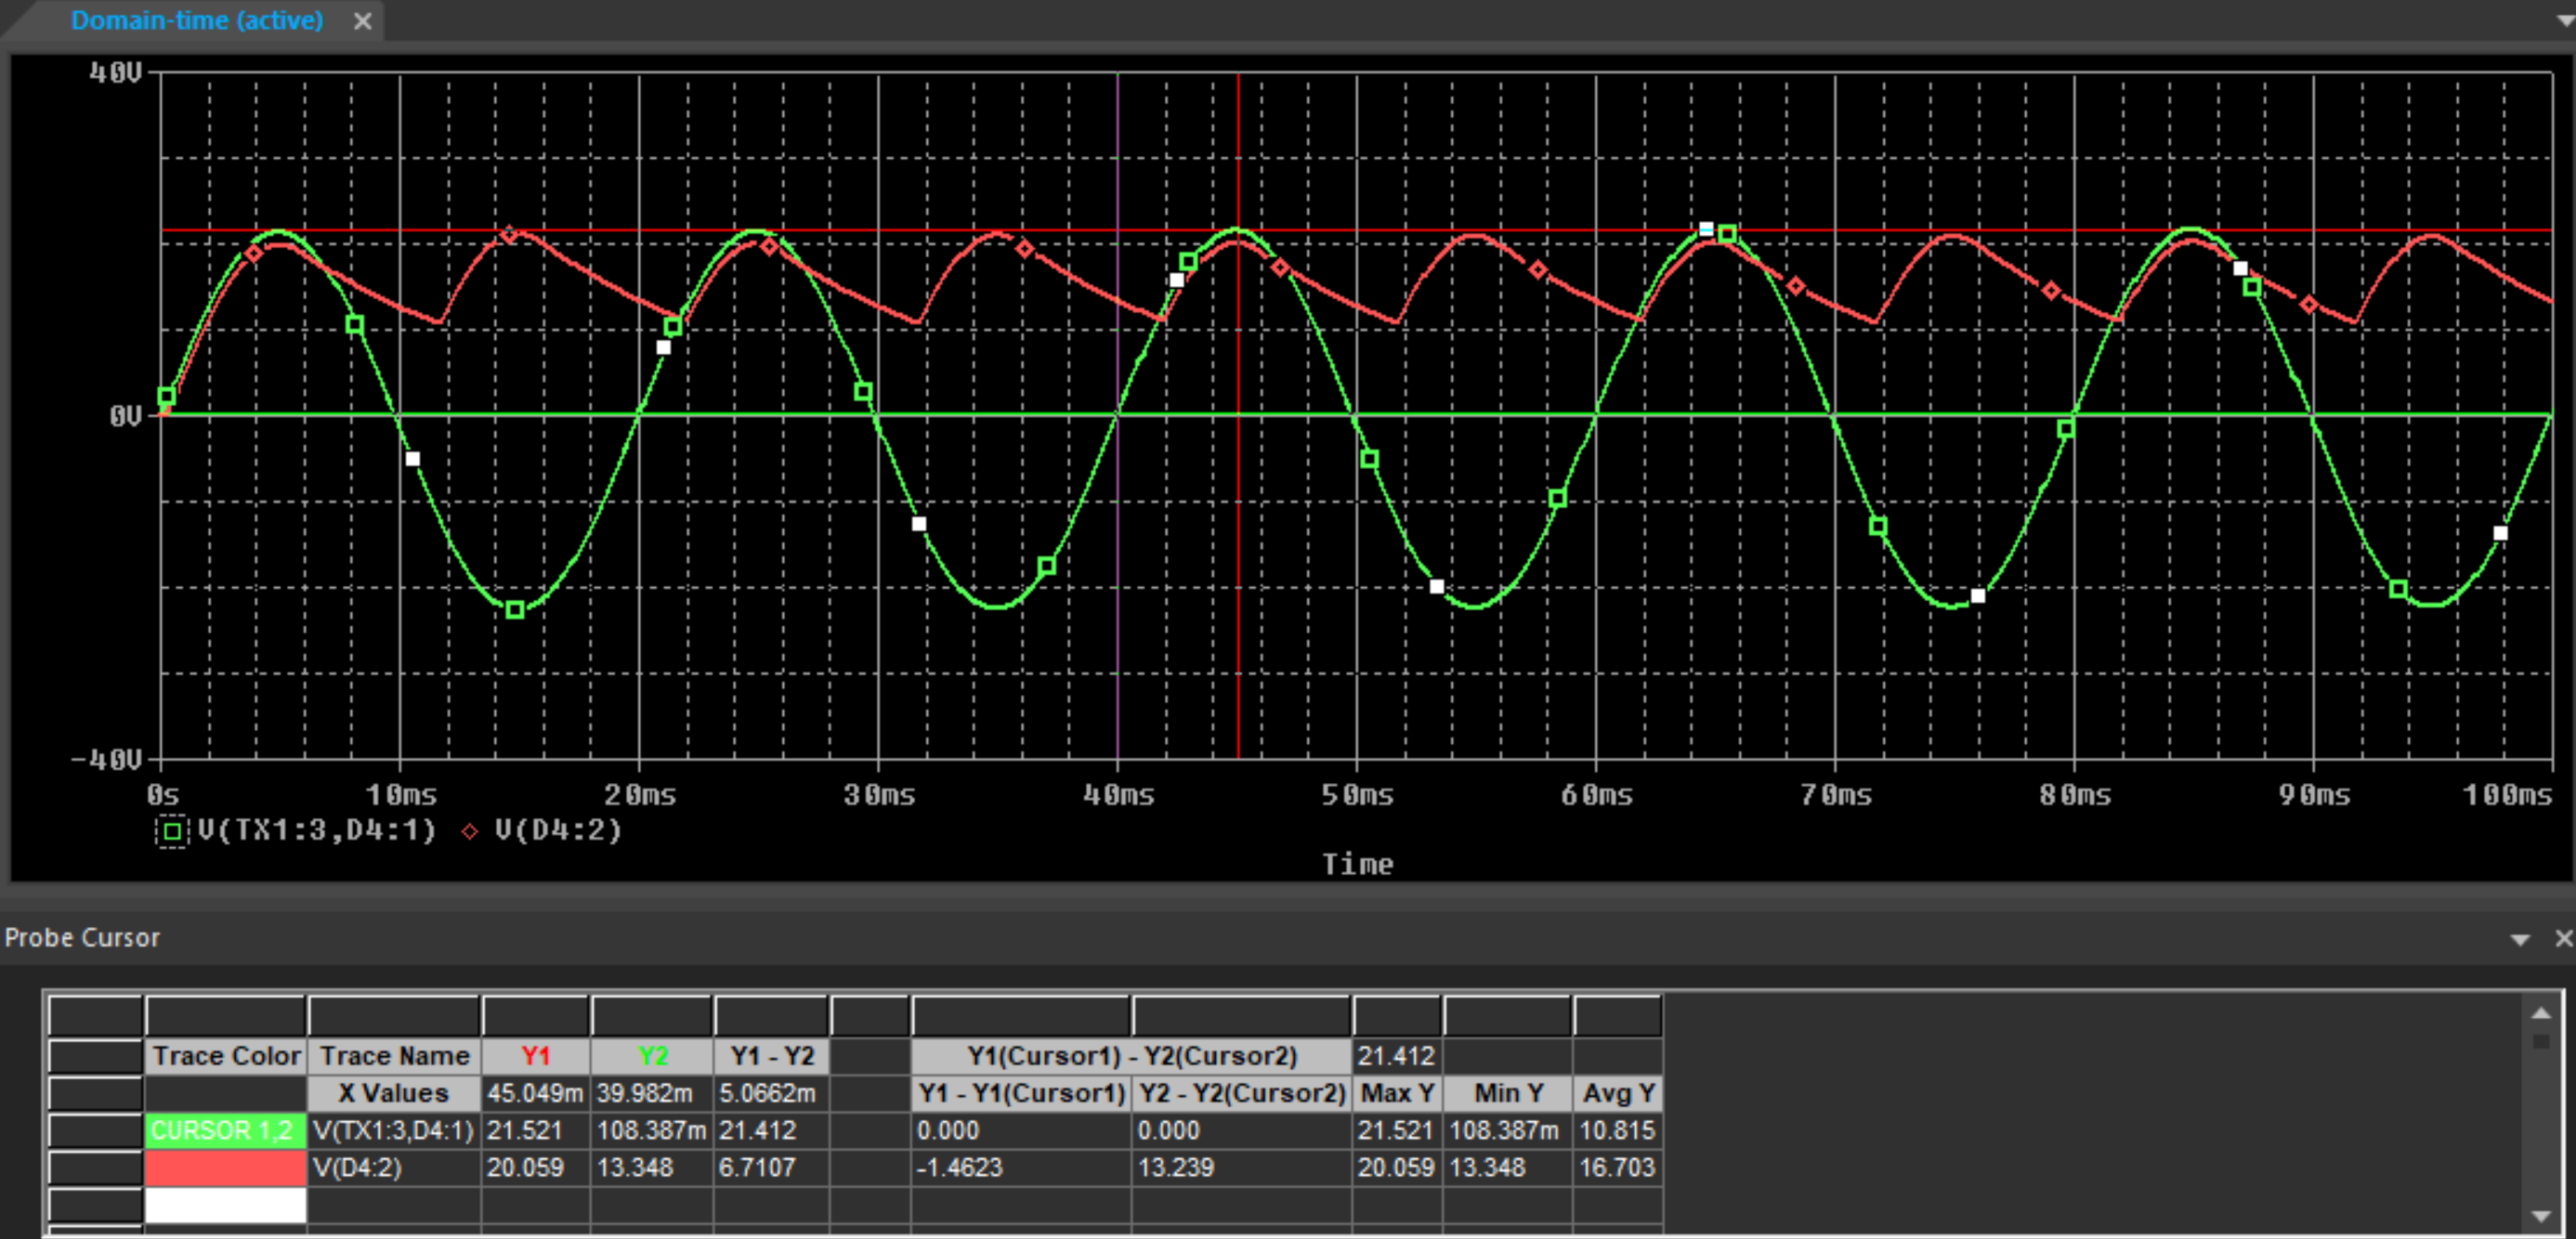
\includegraphics[scale= 0.2]{graphics/ex9/f4.png}
        \caption{Kết quả mô phỏng của mạch trong hình 9.3}
    \end{figure}
    
    \textbf{Ý kiến hoặc giải thích:} Ta có thể thấy rõ sự khác biệt giữa biểu đồ này và biểu đồ trước đó của đồ thị V qua điện trở (màu đỏ) ổn định hơn một chút do quá trình nạp và xả của tụ điện 10 uF. Tại mỗi thời điểm điện áp qua điện trở thấp, tụ điện sẽ phóng năng lượng điện vào mạch. Ngược lại khi điện áp đủ lớn tụ điện sẽ nạp lại điện. Điều này làm cho dòng điện qua điện trở ổn định hơn.
    
    \item \textbf{Step 3:} Thay thế tụ điện 10µF bằng tụ điện 680µF và chạy lại mô phỏng,
    nhận biết sự thay đổi kết quả và giải thích.
 \pagebreak

    \textbf{Kết quả mô phỏng: } 

    \begin{figure}[ht]
        \centering
        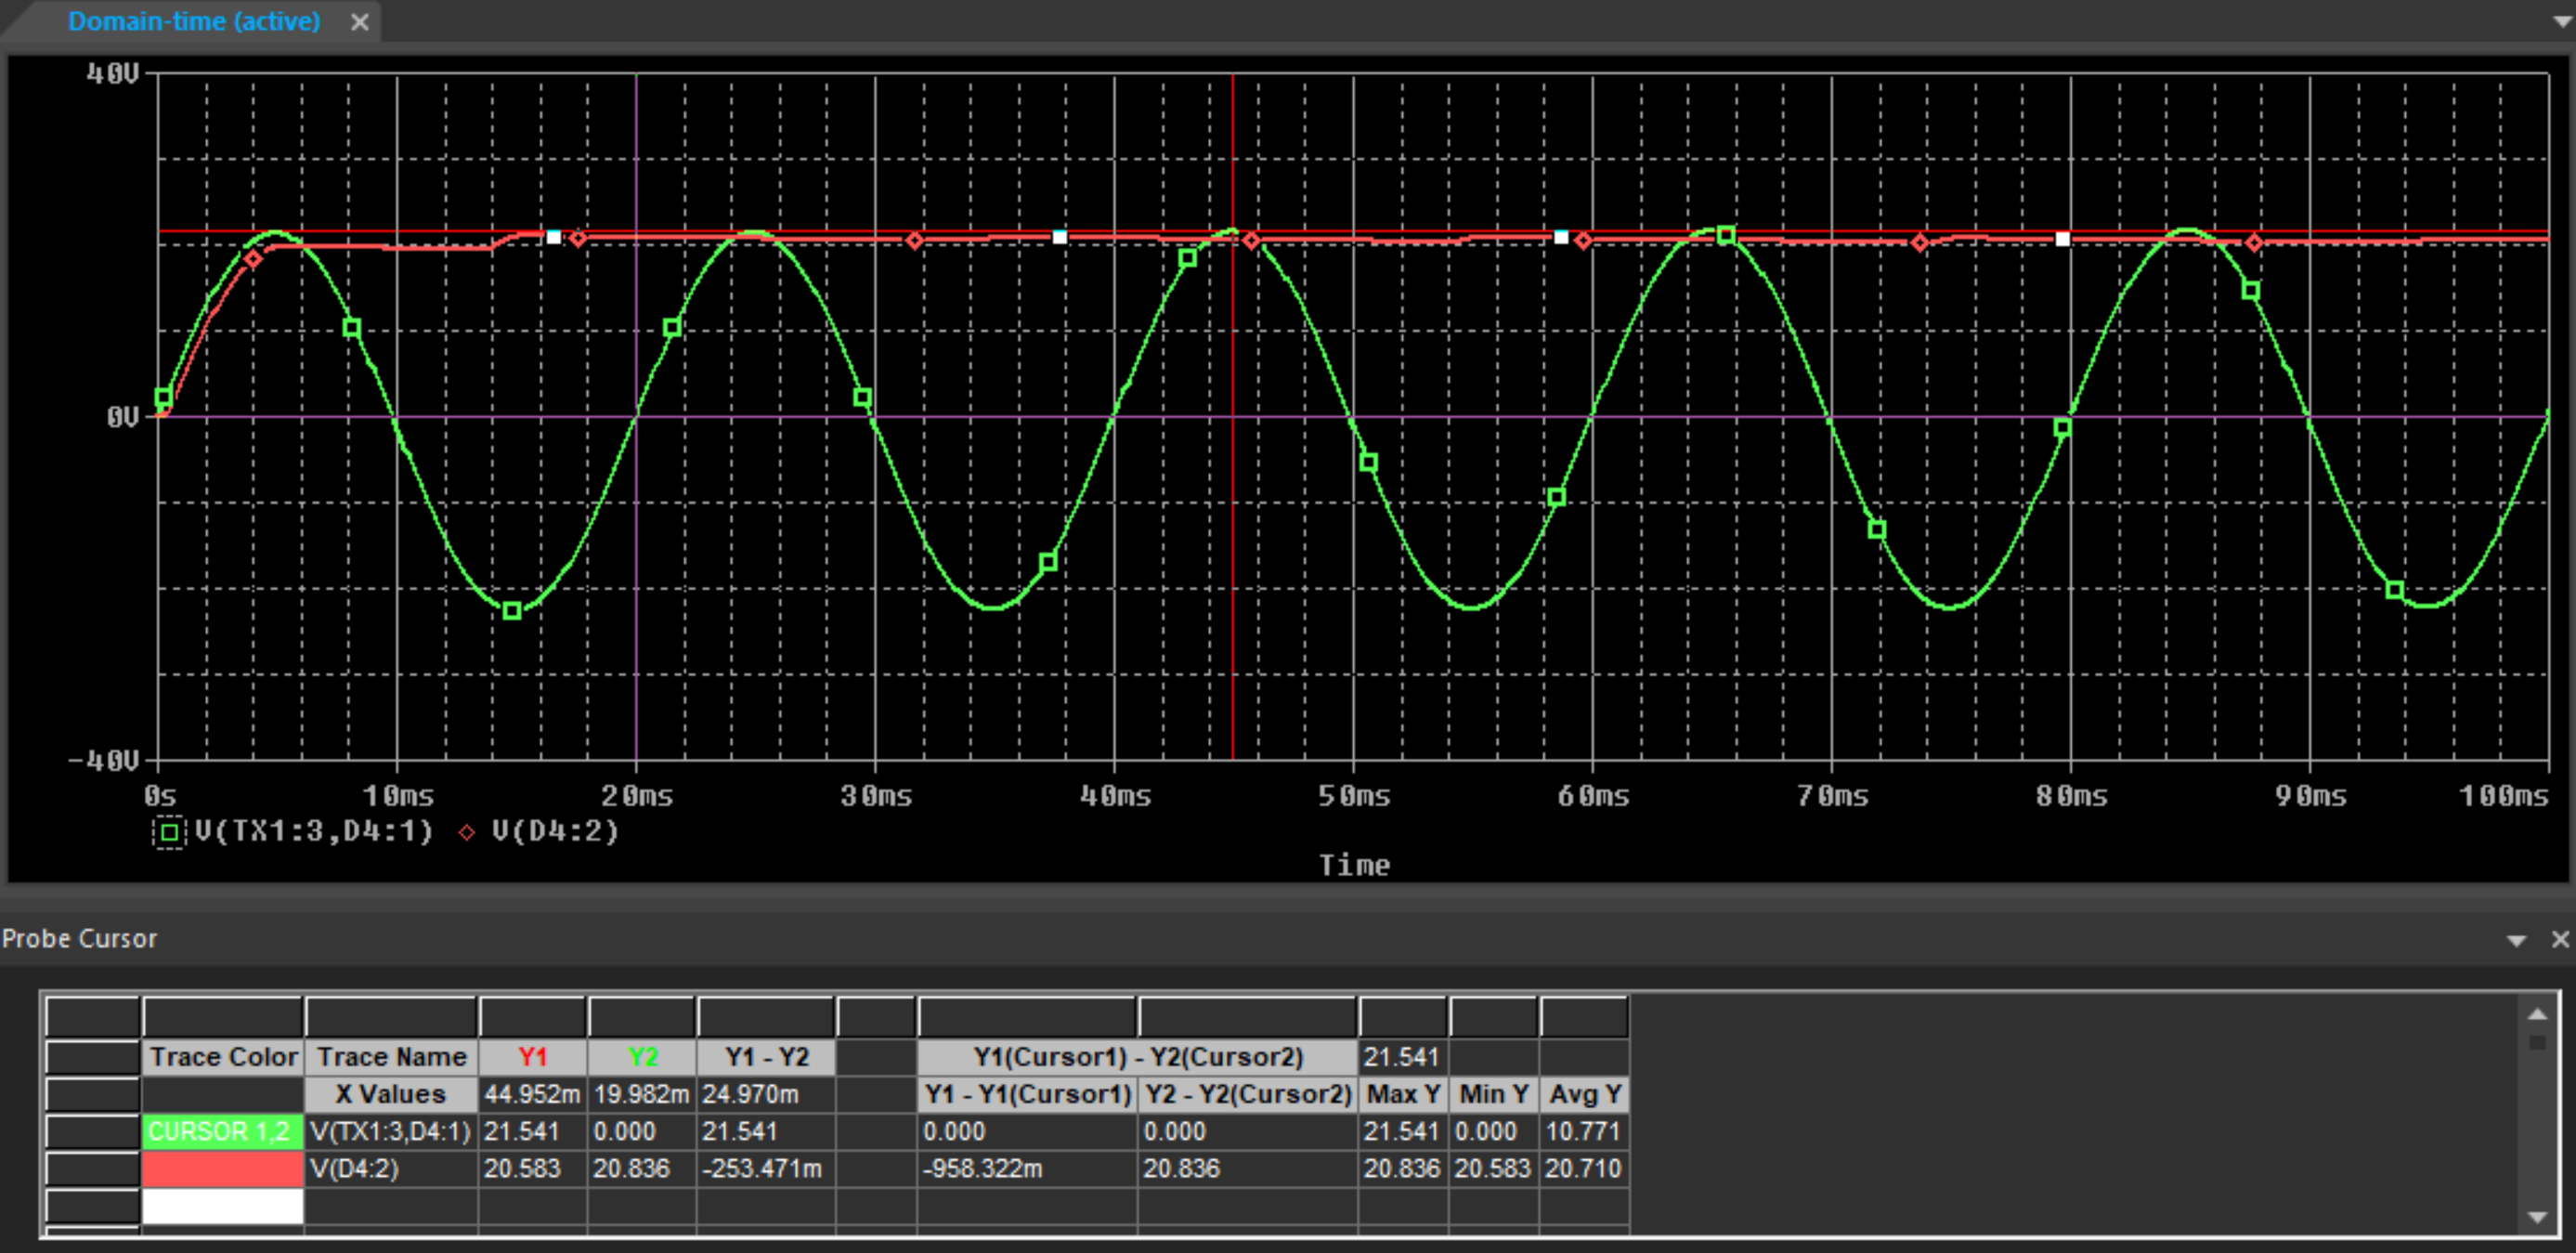
\includegraphics[scale= 0.2]{graphics/ex9/f5.png}
        \caption{Kết quả mô phỏng khi thay giá trị của tụ điện 10µF thành 680µF}
    \end{figure}

    \textbf{Ý kiến hoặc giải thích:} Khi thay giá trị của tụ điện 10µF thành 680µF, ta thấy đồ thị điện áp qua điện trở (màu đỏ) gần như không thay đổi từ chu kì thứ 2 trở đi. Điều này do tụ điện tích điện lớn hơn nên cung cấp điện áp lớn hơn cho mạch.

\item \textbf{Step 4:} Thêm một diode zener như trong Hình 9.6 với các \textit{zener voltage} properties set được đặt thành
22 volt sau đó mô phỏng mạch và nhận xét hoặc giải thích kết quả.

\begin{figure}[ht]
    \centering
    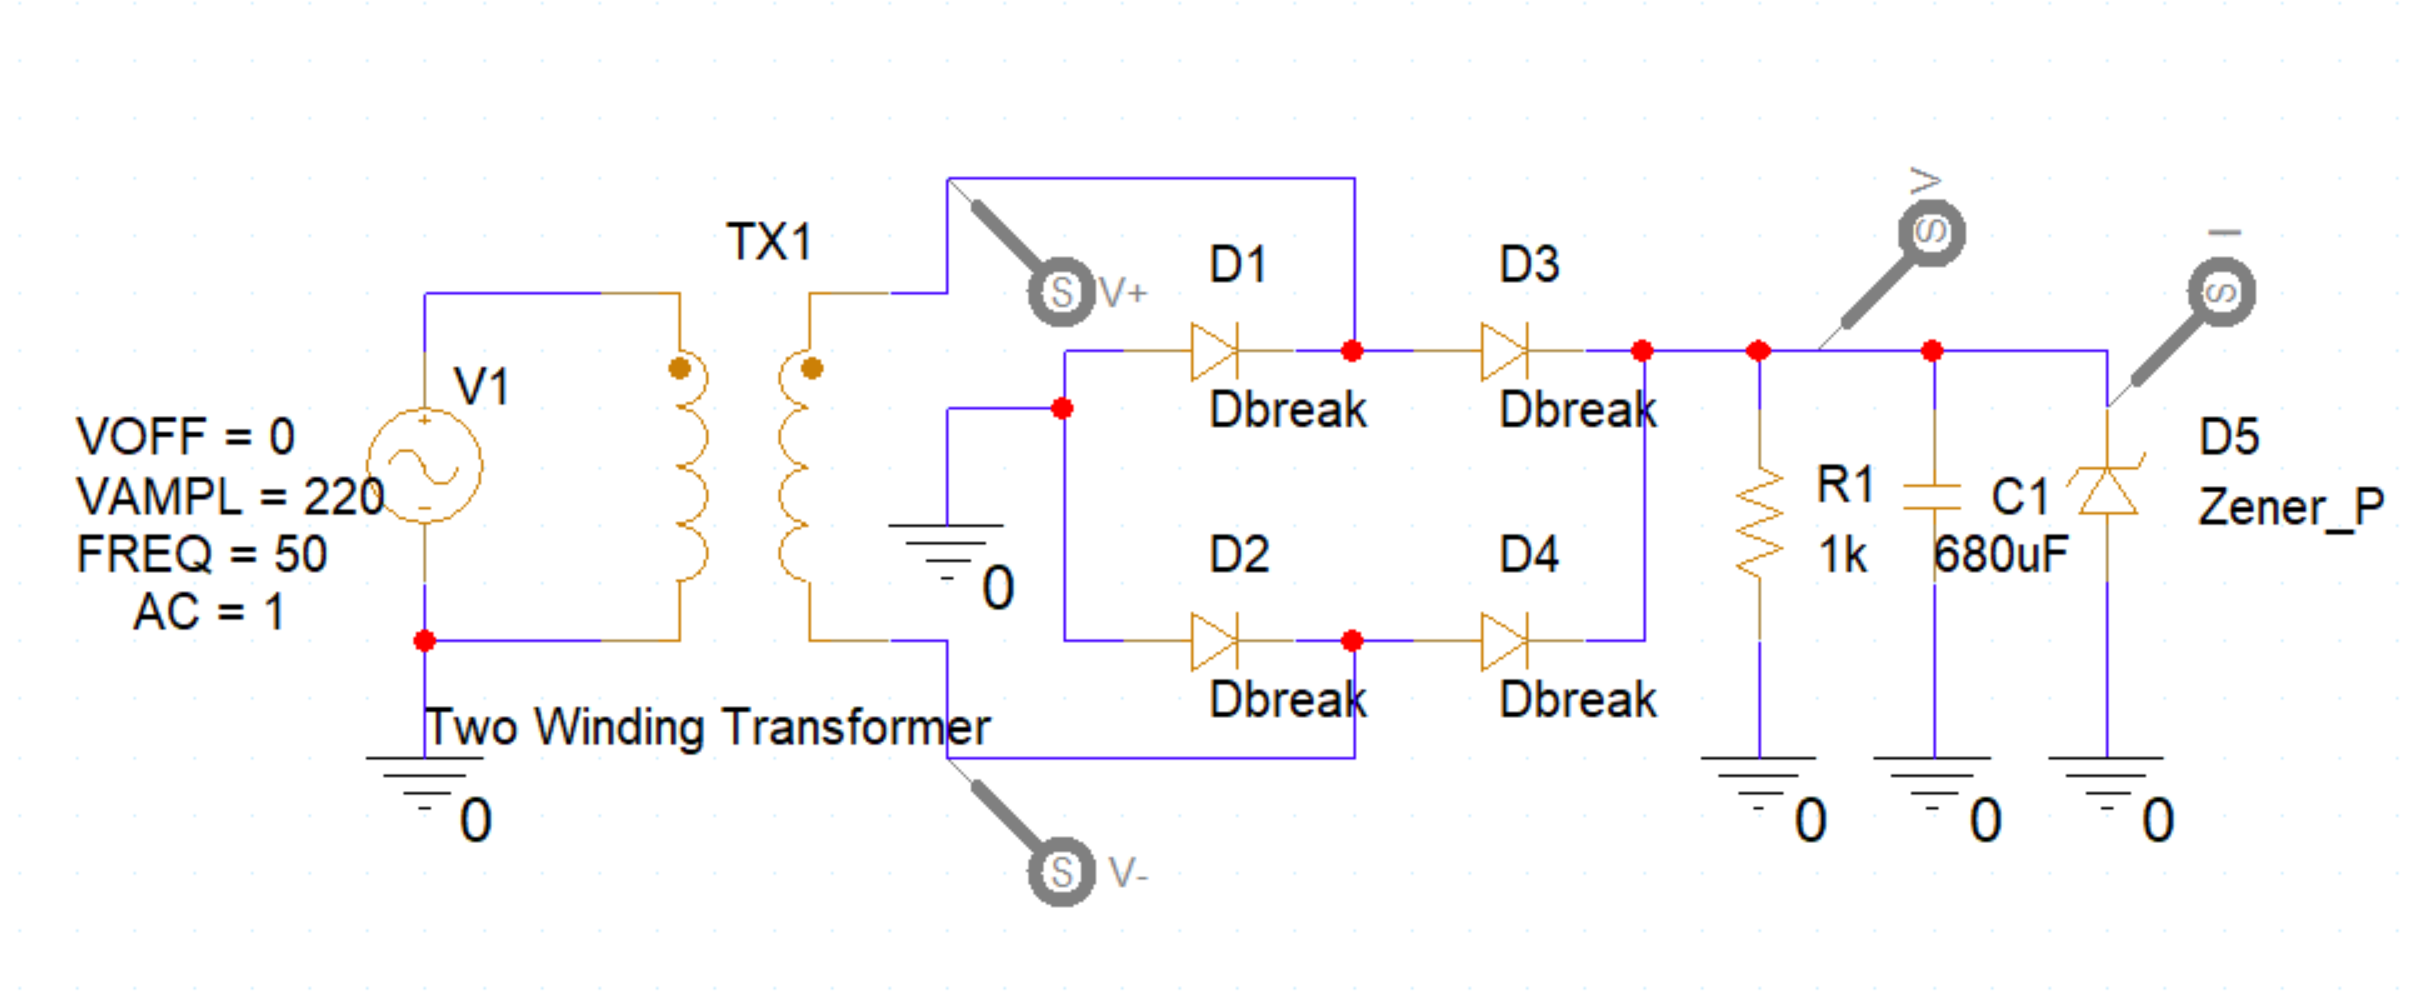
\includegraphics[scale= 0.23]{graphics/ex9/f6.png}
    \caption{Chỉnh lưu điện áp bằng tụ điện và diode zener}
\end{figure}
\pagebreak
\textbf{Kết quả mô phỏng: } 

    \begin{figure}[ht]
        \centering
        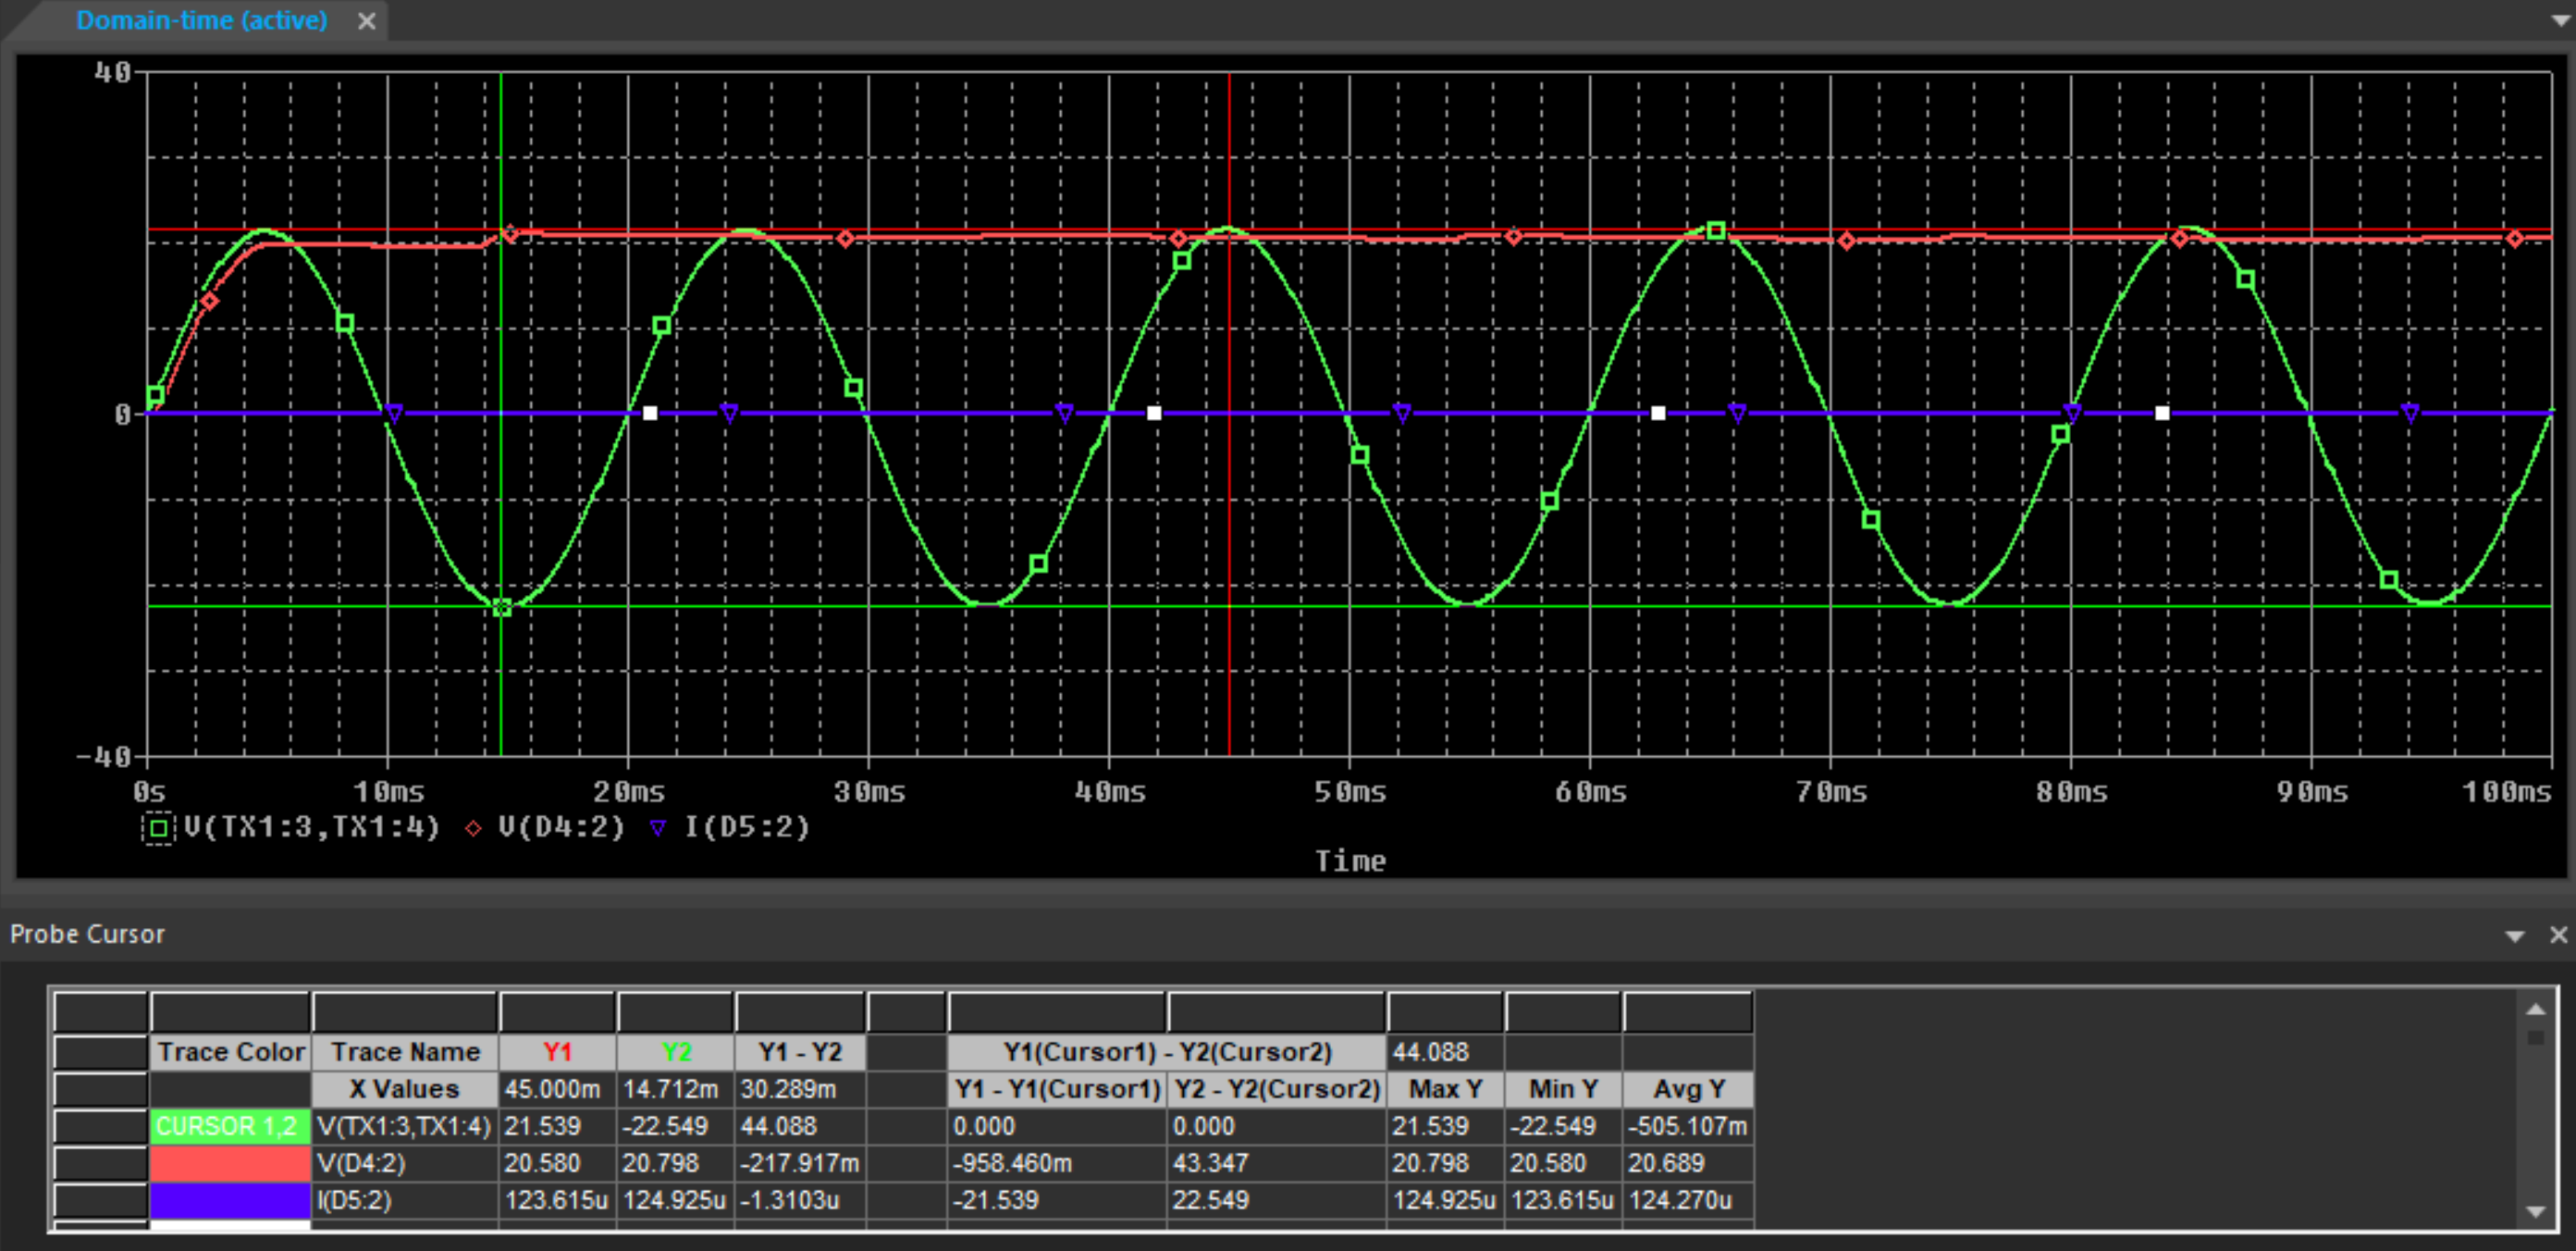
\includegraphics[scale= 0.2]{graphics/ex9/f7.png}
        \caption{Kết quả mô phỏng của hình 9.6}
    \end{figure}

\textbf{Ý kiến hoặc giải thích:} Theo như đồ thị trên, dòng điện đi qua diode zener là 0 V. Điều này có thể được giải thích là do điện áp cao nhất tại R1 là 20,798 (V) trong khi ta đã đặt dòng điện mà diode zener bắt đầu hoạt động là 22 (V). Do vậy mà diode zener không thể hoạt động được.

 \item \textbf{Step 5:} Thay đổi \textit{zener voltage} properties set của diode zener thành điện áp 20 và
 sau đó chạy lại mô phỏng. Nhận xét và giải thích mọi thay đổi trong kết quả.

\pagebreak

 \textbf{Kết quả mô phỏng: } 

 \begin{figure}[ht]
     \centering
     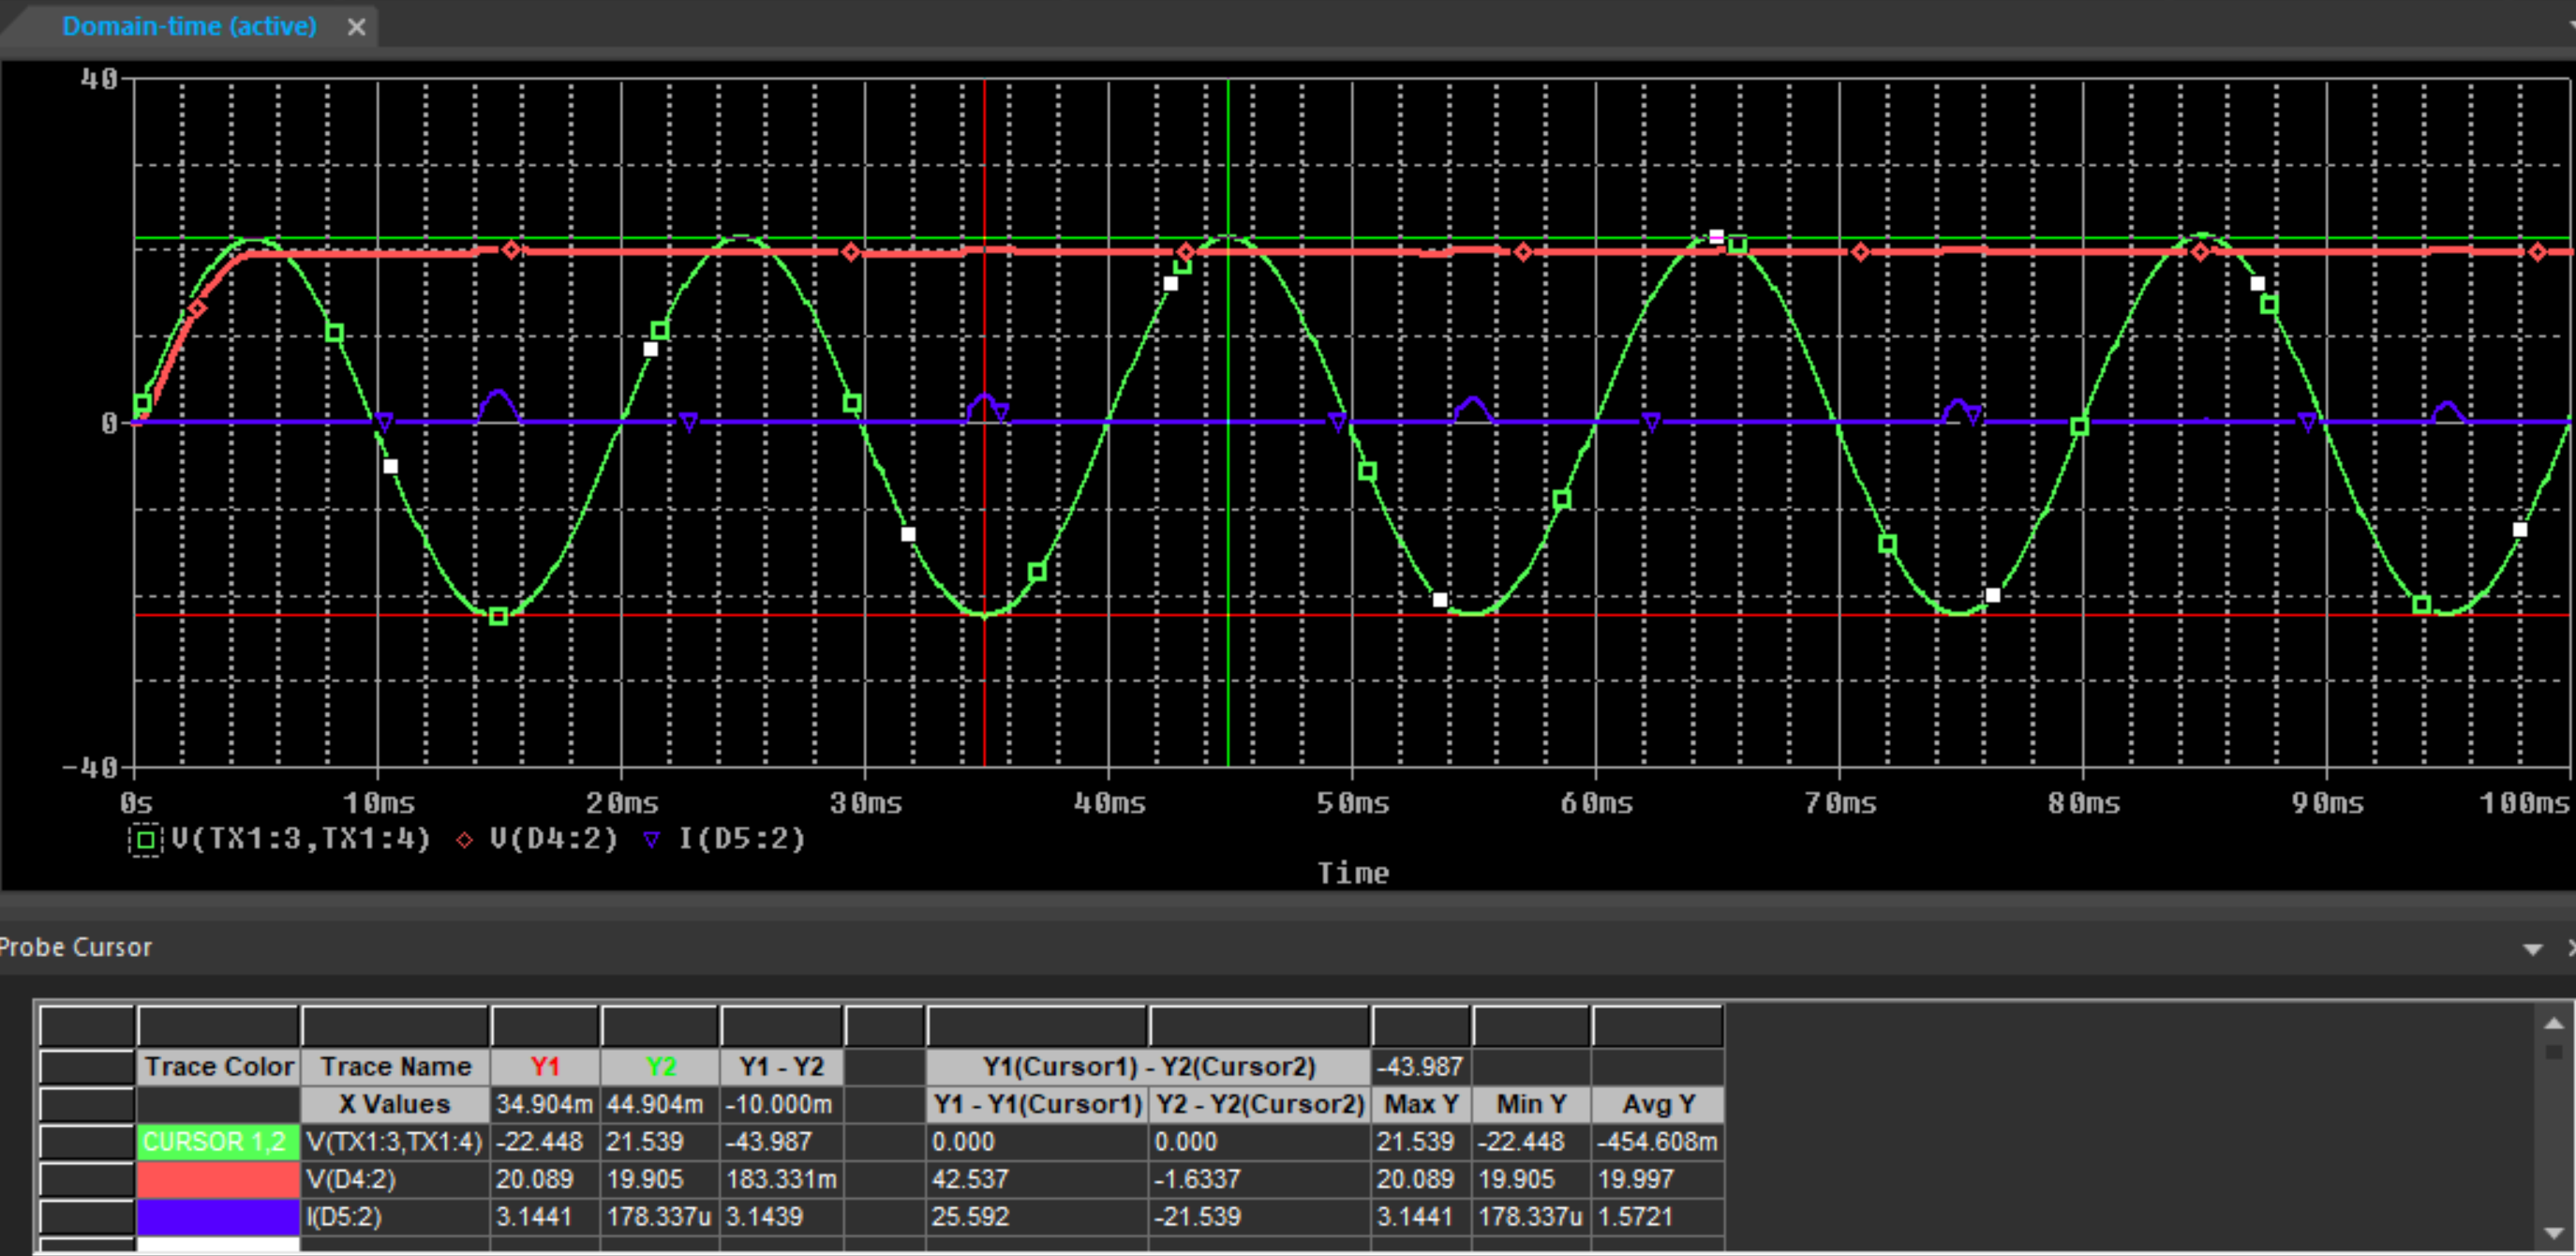
\includegraphics[scale= 0.2]{graphics/ex9/f8.png}
     \caption{Kết quả mô phỏng khi thay giá trị \textit{zener voltage} của diode zener từ 22V thành 20V}
 \end{figure}

 \textbf{Ý kiến hoặc giải thích:} Bởi vì ta đã chuyển dòng điện mà diode zener bắt đầu hoạt động là 20 (V), nên ngay khi điện áp tại R lớn hơn 20 V diode zener bắt đầu hoạt động. Điều này làm cho đồ thị điện áp tại điện trở R1 (màu đỏ)
trở nên ổn định hơn nhưng vẫn còn một chút thay đổi nhỏ.
\end{itemize}